\chapter{绪论}
\label{cha:intro}

\section{引言}

响应理论是实验探测和器件设计的基础。材料的响应指的是在外场的作用下,材料的可观测物理量(用算符$\hat{O}$表示)发生变化的行为。这里的外场一般指的是电场(用$E$表示)或者磁场(用$B$表示)。由于在常见光源中,电磁波中的磁场对材料并没有太大的影响, 因此光场一般可以看成交变电场。由于在施加外场的时候,外场的方向,时间依赖关系,空间依赖关系均可以变化,实验上对材料的探测就有了很多的可变参数,从而探测材料的多种不同性质。实验上的观测物理量则更加多样。传统的可观测物理量有电流电导(霍尔效应\cite{klitzing_new_1980}),磁矩(量子振荡\cite{SdH,dHvA}),极化(铁电回线\cite{cohen_origin_1992})等等。近年来,人们开始尝试探索电子的新的自由度,由此诞生了一些新的物理可观测量,例如自旋流(自旋霍尔效应\cite{hasan2010,qi2011}),谷极化流(谷霍尔效应\cite{xiao_coupled_2012})等。这些手段极大地丰富了凝聚态实验的种类,并且对工程应用也有极大的价值。


由于实验探测的目的主要是了解材料本身的性质,因此实验施加的外场往往较小。在这样的背景下,可观测量偏离平衡态的大小($\delta\langle\hat{O}\rangle$)经常以外场场强进行小量展开。除非对称性禁止,小量展开的最低阶往往是线性的($\delta\langle\hat{O}\rangle \propto E$或者$B$),这样的响应称之为线性响应。随着实验技术的发展和实验目的的变化,人们有时也对研究的样品材料施加强场,以期获得高阶的响应,这样的响应统称为高阶响应。其中,二阶响应是最容易被实验观测到的,也是人们研究最多的对象。

一般而言,由于电子之间存在着交换关联作用,计算一个系统对外场的响应尤其是高阶响应是一件比较困难的事情。幸运的是,对于非强关联体系,基于密度泛函理论的独立粒子近似就能够较好地预测实验结果。因此,本文的理论分析基本基于独立粒子近似,而计算手段则采用基于密度泛函理论的能带论。

在独立粒子近似下,计算材料的响应有很多中手段,最流行的两种手段是格林函数和准经典运动方程\cite{xiao_berry_2010}。这两种手段在输运理论中都取得了巨大的成功。格林函数,尤其是非平衡格林函数,应用面更加广泛。而准经典运动计算更加简单更加直观。下面本文将对准经典运动方程做一个简要介绍,然后列举出一些本文将会探讨的响应现象。首先是位移电流\cite{sipe_second-order_2000,von_baltz_theory_1981},位移电流是布洛赫电子对电场响应的例子。其次是布洛赫电子在静磁场中的行为。这些响应现象将会是本文研究的中心。

\section{准经典运动方程}

准经典运动方程是基于波包的动力学。波包指的是用同一条能带上的多个布洛赫波叠加得到的量子态,波包不具有确定的晶格动量,但是具有良好定义的位置算符的本征值。具体来说,波包$|W\rangle$定义为
\begin{equation}
|W\rangle=\int d\bk w(k, t)|\phi_n(\bk)\rangle.
\end{equation}
其中,$\phi_n$是第$n$条带上的布洛赫波函数,而$w(\bk,t)$则是叠加的权重。一般而言这个权重是局域在某一个晶格动量上的
\begin{equation}
\bk_c = \int dk \bk w(\bk,t).
\end{equation}
此时,这个波包的位置是具有良好定义的期望值的
\begin{equation}
\boldsymbol{r}_c = \left. -\frac{\partial}{\partial \bk} \arg w(\bk, t) + \berry_n(\bk)\right|_{\bk=\bk_c}.\label{semi-rc}
\end{equation}
这里的$\boldsymbol{\berry}_n(\bk)=i \langle u_n(\bk)|\nabla_{\bk}|u_n(\bk) \rangle$被称为贝里联络,$u_n(\bk)$则是布洛赫波的周期性部分。

$\bk_c$ 和 $\br_c$ 是波包的重要性质。在经典的牛顿力学理论中,这两个量分别对应粒子的动量和位置。由于不确定原理,这两个量在量子力学中仅仅是期望值。 在外电场和磁场很小的情况下,$\bk_c$ 和 $\br_c$的运动方程是(下标$c$省略)
\begin{align}
	\dot{\br} &= \frac{\partial \epsilon_M(\bk)}{\hbar\partial \bk}-\dot{\bk}\times\boldsymbol{\Omega}(\bk)\nonumber\\
	\hbar\dot{\bk} &= -e\boldsymbol{E}-e\dot{\br}\times\boldsymbol{E}.\label{semi-eqn}
\end{align}
这里的$e$是(正的)基本电荷的大小。波包运动的方程和经典的牛顿运动方程非常相似,但是存在着几个修正,下面我们一项一项分析其修正。

第一个修正来自于轨道磁矩,和牛顿力学中的粒子不同,波包并没有确定的位置,波包的波函数在实空间里面是延展的。因此波包可以围绕这自己的中心旋转,这样的旋转会带来不为0的轨道磁矩,在磁场中,轨道磁矩会贡献额外的能量,因此第一项修正为$\epsilon_M(\bk)=\epsilon(\bk)-\boldsymbol{M}(\bk)\cdot\boldsymbol{B}$。这里的$\epsilon(\bk)$是没有外场下的布洛赫波的能量,而轨道磁矩的计算表达式为
\begin{equation}
\boldsymbol{M}(\bk) = -i\frac{e}{2\hbar}\langle\nabla_{\bk}u|\times [\hat{H}(\bk)-\epsilon(\bk)]|\nabla_{\bk}u\rangle.
\end{equation}
可以看到轨道磁矩并不和波包的具体形式有关,只和体的波函数相关。这给计算带来了巨大的便利。

第二个修正来自于贝里曲率,这又是一项超越经典力学的修正项。经典力学中粒子的运动是用实数描述的,而量子力学中的波函数则必须使用复数来描述,复数和实数的巨大差异就来源于复数存在相位。贝里曲率则来源于波包运动过程中产生的几何相位。贝里曲率的定义是
\begin{equation}
\boldsymbol{\Omega}(\bk) = \nabla\times\boldsymbol{\berry}(\bk).
\end{equation}
它贡献了式\ref{semi-eqn}中的反常速度项(第一行右手边的第二项)。

式\ref{semi-eqn}刻画了波包运动过程中的信息,固体作为一个电子气的集合,我们还需要知道波包在相空间($\bk-\br$空间)的分布情况。在没有磁场的情况下,相空间的态密度是均匀分布的。但是在有磁场的情况下,相空间的态密度则会需要进行修正。这个态密度是
\begin{equation}
D(\br,\bk)=\frac{1}{(2\pi)^d}(1+\frac{e}{\hbar}\boldsymbol{B}\cdot\boldsymbol{\Omega}).\label{semi-dens}
\end{equation}
这里$d$是空间的维度。

式\ref{semi-eqn}和式\ref{semi-dens}是准经典波包理论的重要结果。这两个式子结合在一起,可以预测固体的大量性质,这些预言在实验上获得了巨大的成功。

\section{位移电流}

位移电流\cite{tan_shift_2016}是本文的研究重点之一,这一小节我们对位移电流做一个简单的介绍。

位移电流是一种光伏效应,指的是在线性偏振光的照射下,没有空间反演对称性的材料产生自发直流电的现象。目前广泛应用的光电池往往基于$p-n$结,是一种界面效应。与此相反,位移电流来源于体的能带结构,被称为体的光伏效应。

位移电流是一种二阶效应,具体来说,位移电流$\boldsymbol{J}$可以表达为
\begin{equation}
J^\alpha = \sigma^{abb}(\omega) E^a(\omega) E^b(\omega).
\end{equation}
这里的$a$和$b$是笛卡尔方向的指标,$\omega$是光场的频率,$\sigma^{abb}$被称为位移电导。

位移电流的起源是电子在光场的作用下从价带跃迁到导带时发生的位置变化,位移电导计算表达式为
\begin{equation}
\sigma^{abb}=-\frac{2\pi e^3}{\hbar^2}\int \frac{d\bk}{(2\pi)^3}\sum_{n,m}f_{mn}|r^b_{mn}|^2 R_{nm}^{ab} \delta(\omega_{nm}-\omega),\label{shift-expr}
\end{equation}
这里的积分区域为第一布里渊区,$n,m$是能带标号,$f_{mn}=f_m-f_n$是费米分布的差,$r_{mn}(\bk)=i \langle u_m(\bk)|\nabla_{\bk}|u_n(\bk) \rangle$是贝里联络的非对角项,$\omega_{nm}=\omega_n-\omega_m$是能带能量的差($\epsilon_n=\hbar\omega_n$), 而$R_{nm}^{ab}$具有长度的单位,被称为位移矢量。位移矢量和式\ref{semi-rc}紧密相关,具体形式为
\begin{equation}
R_{nm}^{ab}=\partial_a \phi_{mn}^{b}-\berry_m^a+\berry_n^a,
\end{equation}
其中$\phi_{mn}^{b}$是$\berry_{mn}^{b}$的相位。位移矢量的物理阐释就是电子从带$m$跃迁到带$n$发生的位置变化的大小。假设一个波包原先在带$m$上,其权重函数为$w_m(\bk,t)$, 假设光作为微扰项加入本系统中,采用极化子近似,那么微扰哈密顿量就是$\hat{H}_D=A^b\hat{p}^b$,其中$\boldsymbol{A}$是矢势。根据含时的一阶微扰论,跃迁到能带$n$上的权重函数正比于$w_n(\bk, t)\propto p^b_{nm}w_m(\bk, t)$。考虑到$p_{nm}$和$r_{nm}$的相位是锁定在一起的(相差$\pi/2$),我们就可以根据式\ref{semi-rc}计算出跃迁前后的位置平均值的差。这个差就是位移矢量。

位移电导还有另一个等价的表达式,这个表达式更加适用于数值计算
\begin{equation}
	\sigma^{abb}(\omega)=\frac{2\pi e^{3}}{\hbar^{2}}\int\frac{d^{3}\bk}{(2\pi)^{3}}\sum_{n,m}f_{nm}I_{nm}^{abb}\delta(\omega_{nm}-\omega),\label{eq:shift-current}
\end{equation}
其中
\begin{equation}
I_{nm}^{abb}=\text{Im}[r_{mn}^{b}r_{nm;a}^{b}],\label{eq:shift-integrand}
\end{equation}
其中$r_{nm;a}^{b}=\partial_{k_{a}}r_{nm}^{b}-i(\berry_{n}^{a}-\berry_{m}^{a})r_{nm}^{b}$被称为贝里相位的广义导数。

位移电流只有在空间反演破缺的情况下存在,在没有空间反演破缺的材料中,式\ref{shift-expr}被积函数在$\bk$和$-\bk$处严格相反,所以积分结果严格为零。除了空间反演对称性以外,还有别的对称性可以禁止位移电导的某些分量。一般而言,$\berry$和位置算符$\hat{\br}$具有相同的对称变换规则。比如,既然$\hat{T}\hat{\br}\hat{T}^{-1}=\hat{\br}$($T$是时间反演操作),那么在具有时间反演对称的晶体中就有$\berry_{nm}(\bk)=\berry_{nm}^*(-\bk)$。既然$\hat{\inv} \hat{\br} \hat{\inv}^{-1}=-\hat{\br}$($\inv$是空间反演操作),那么具有空间反演对称性的材料就会有$\berry_{nm}(\bk)=-\berry_{nm}(-\bk)$。这样的关系可以用来分析位移电导在各种对称性下的变换。注意,由于贝里联络可以出现相位不定性。因此上面的等式都是在选择了一定的相位规范下成立的。

\begin{figure}
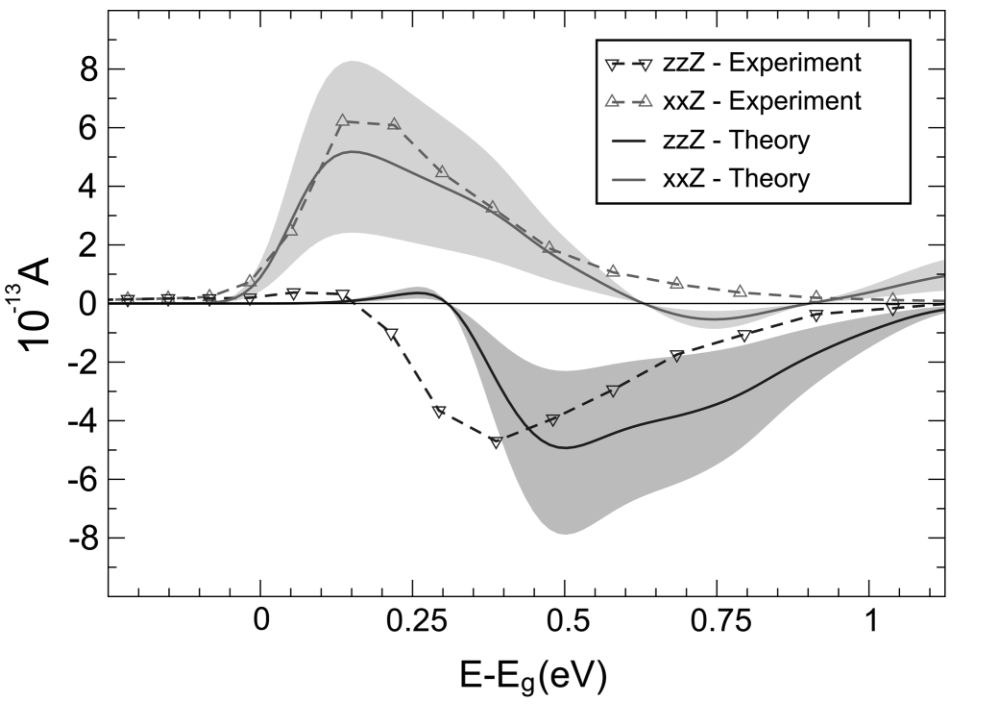
\includegraphics[width=1.0\textwidth]{../figures/young-shift.png}
\caption{BaTiO$_3$的不同方向的位移电流的理论和实验值\cite{koch_anomalous_1976}对比。实线是理论值,虚线是实验值。灰色部分是由于实验样品尺寸的不确定性导致的卢纶值的不确定范围。本图来自文献\onlinecite{young2012}。 注意:该文和本论文采用的符号不一致。本文中的$\sigma^{\alpha\beta\beta}$相当于文献\onlinecite{young2012}中的$\sigma^{\beta\beta\alpha}$(见图例)。\label{young-shift}}
\end{figure}

最早的和实验进行对比的位移电流的计算出现2012年,Steve Young等人\cite{young2012}通过第一性原理方法计算了BaTiO$_3$的位移电流。BaTiO$_3$是典型的铁电材料,具有较大的极化。Steve Young等人和更早期的实验进行了对比,得到了相对比较满意的结果(图\ref{young-shift})。

自此之后,出于实际应用的目的,人们开始探索什么样的材料能够具有较大的位移电流。Cook等人\cite{cook_design_2017}通过建立紧束缚模型并且调节模型参数,推荐了单层GeS作为具有较大位移电流的材料。Fregoso等人\cite{fregoso_quantitative_2016}提出,在一定条件下,位移矢量的平均值就是导带和价带的极化差,指出了极化和位移电流存在着非常紧密的关系。但是在实际计算中,人们发现位移电流并不是随着极化的增长单调上升的。后来,Tan等人\cite{tan_upper_2017}提出位移电流存在上限,这个上限正比于紧束缚模型的跃迁参数和带隙的比值的平方。但是这个上限仍然是理想化模型化的,实际材料中的紧束缚模型跃迁参数并不是一个容易确定的数值。Tan等人还尝试对位移电流进行了高通量计算,从中找出了一些位移电流比较大的材料。


\section{布洛赫电子的磁性质}

与电场相比,布洛赫电子的磁性质的研究要困难许多。在一定的规范下,电场可以不破坏晶体的离散平移对称性。但是无论选取什么规范,磁场一定会破坏晶体的离散平移对称性。因此,布洛赫电子在磁场中的运动往往在磁场非常小的情况下进行近似。这个近似在绝大部分实验条件下都是非常合理的。磁场作为小量的理论在这里被称为准经典理论。

人们早已知道,自由电子在磁场中的能级是分立的,这些能级被称为朗道能级。在晶体中,电子的表现是相似的。在费米面没有穿过布里渊区边界的情况下,电子的能级也是分立的,这些能级同样被称为朗道能级。Peierls-Onsager-Lifshitz准经典理论\cite{lifshitz_kosevich,lifshitz_kosevich_jetp}就是一个求解磁场中布洛赫电子的朗道能级和朗道能级波函数的理论,随着磁场变小,Peierls-Onsager-Lifshitz准经典理论越来越精确。Peierls-Onsager-Lifshitz准经典理论的强大之处在于,这个理论仅仅需要知道零场下的电子的能带结构信息,就可以预测出弱磁场下的晶体的各种性质。我们在本文中仅仅讨论等能面闭合的情况,等能面穿过布里渊区的问题留到以后进行研究。由于磁场并不破坏沿着磁场施加方向的离散平移对称性,三维材料在磁场中可以看成二维能带的简单组合。因此在本文中,如果没有特殊说明,我们只讨论二维材料。另外,如果没有特殊说明,我们默认磁场沿着$-z$方向,这样的设定让电子型的载流子会(从$z$方向看过去)逆时针作回旋运动。

在最简单的物理图像下,电子在磁场中会沿着等能面做回旋运动,此时这个电子被称为磁振子。磁振子的运动方程为
\begin{equation}
\hbar\dot{\bk}=-\frac{e}{\hbar}\nabla_{\bk}\epsilon\times\boldsymbol{B}.
\end{equation}
这里$\epsilon$是能带能量。这个回旋运动的周期我们称为磁振子的周期,记为$T_c$.
\begin{equation}
T_c=\frac{1}{\hbar l^2 |dS/dE|}.
\end{equation}
这里,$S$是能量为$E$的等能面的面积。我们同时在这里引入磁长度的概念
\begin{equation}
l=\sqrt{\frac{\hbar}{eB}}.
\end{equation}
磁长度的物理含义是电子在磁场中运动,大概获得$2\pi$的相位所需要运动的长度。在磁场是一个小量的假设下,磁长度$l$是一个大量。磁振子的能量定义为
\begin{equation}
\epsilon_c=\frac{h}{T_c}=\hbar \omega_c.
\end{equation}
磁振子能量刻画了朗道能级的间隔。除此之外,我们还要引入磁振子质量$m_c$
\begin{equation}
\epsilon_c = \hbar^2/m_c l^2.
\end{equation}
对于自由电子,$m_c=m_0$,其中$m_0$就是自由电子的质量。


更加严格的理论则是基于有哈密顿量理论\cite{rotheffham}。这个理论将哈密顿量中的磁场小量展开,在一组合适的基下表示出来。有效哈密顿量理论既可以在实空间表述,也可以在$\bk$空间表述。在零阶近似下,有效哈密顿量在$\bk$空间的表述叫做Peierls替换:将能带能量$\epsilon(\bk)$直接替换为$\epsilon(\bK)$,这里,$\bK=\bk+(e/\hbar)\boldsymbol{A}(i\nabla_{\bk})$。这里的$\epsilon(\bK)$是一个算符,作用在$\bk$空间的波函数上,定态薛定谔方程就变成了
\begin{equation}
\epsilon(\bK)f(\bk)=Ef(\bk).
\end{equation}
这个定态薛定谔方程可以用WKB近似得到近似解。近似解最方便的表达方式是量子化条件,量子化条件是一个关于能量$E$和磁场$B$的方程,这个方程的解就是朗道能级。在零阶近似下,量子化条件是
\begin{equation}
l^2 S=2\pi n+\pi.
\end{equation}
这里的$n$是整数,$\pi$被称为Maslov相位,来自于WKB的量子修正。Maslov相位等于$\pi$仅仅在等能面可以连续变化为圆的时候才成立。这个量子化条件E和B的依赖分别来自于等能面面积$S$和磁长度$l$.

近年来,随着凝聚态中拓扑性质的发现,人们逐渐意识到除了动力学相位之外,几何相位\cite{berry_quantal_1984}同样非常重要。几何相位在量子化条件中贡献的是一阶项。事实上,除了几何相位之外,量子化条件中的一阶项还由轨道磁矩和自旋磁矩贡献。在磁场中,这些磁矩会带来额外的能级移动,从而产生额外的相位。

这些额外的能量在有效哈密顿量里面表现为修正项$\mathfrak{h}_1(\bK)$, 这里。
\begin{equation}
\mathfrak{h}_1(\bk)=B(M^z-g_s\mu_Bs^z/\hbar+e\epsilon^{\alpha\beta}\berry^\beta v^\alpha),
\end{equation}
其中$M^z$是前述的轨道磁矩,$g_s$是自由电子的$g$因子,$\mu_B$是波尔磁子,$s^z$是$z$方向的自旋,$\boldsymbol{v}$是能带速度。

在考虑进这些修正之后,量子化条件改变为
\begin{equation}
l^2 S+\lambda = 2\pi n +\pi\label{single-quan},
\end{equation}
其中
\begin{equation}
\lambda = il^2\oint \frac{\mathfrak{h}_1}{\hbar v^x} dk^y.
\end{equation}
这里积分路径逆时针沿着磁振子轨道。注意$\lambda$和磁场无关,仅仅和能量有关。


以上介绍的是单能带电子的量子化条件。单能带电子指的是在等能面上这个能带处处不简并,并且能隙全部都远大于磁振子能量$\epsilon_c$。如果这个条件不成立,那么量子化条件就需要做出相应的改变。一个典型的情况是能带在布里渊区的一个小区域和其他能带接近简并,这样的情况就会发生磁隧穿现象。如果一个能带处处和其他能带接近简并,那么量子化条件需要做更加复杂的修改,这是本文的研究重点之一。

\subsection{量子振荡}

在磁场中的材料的各种性质会随着磁场的倒数$1/B$周期性振荡,这样的振荡现象被称为量子振荡。最著名的两个量子振荡是de Haas-van Alphen(dHvA)振荡\cite{dHvA}和Shubnikov–de Haas(SdH)振荡\cite{SdH}。dHvA振荡指的是磁矩(或者磁化率)随着磁场的振荡,而SdH振荡指的是电阻随着磁场的振荡。

\begin{figure}
	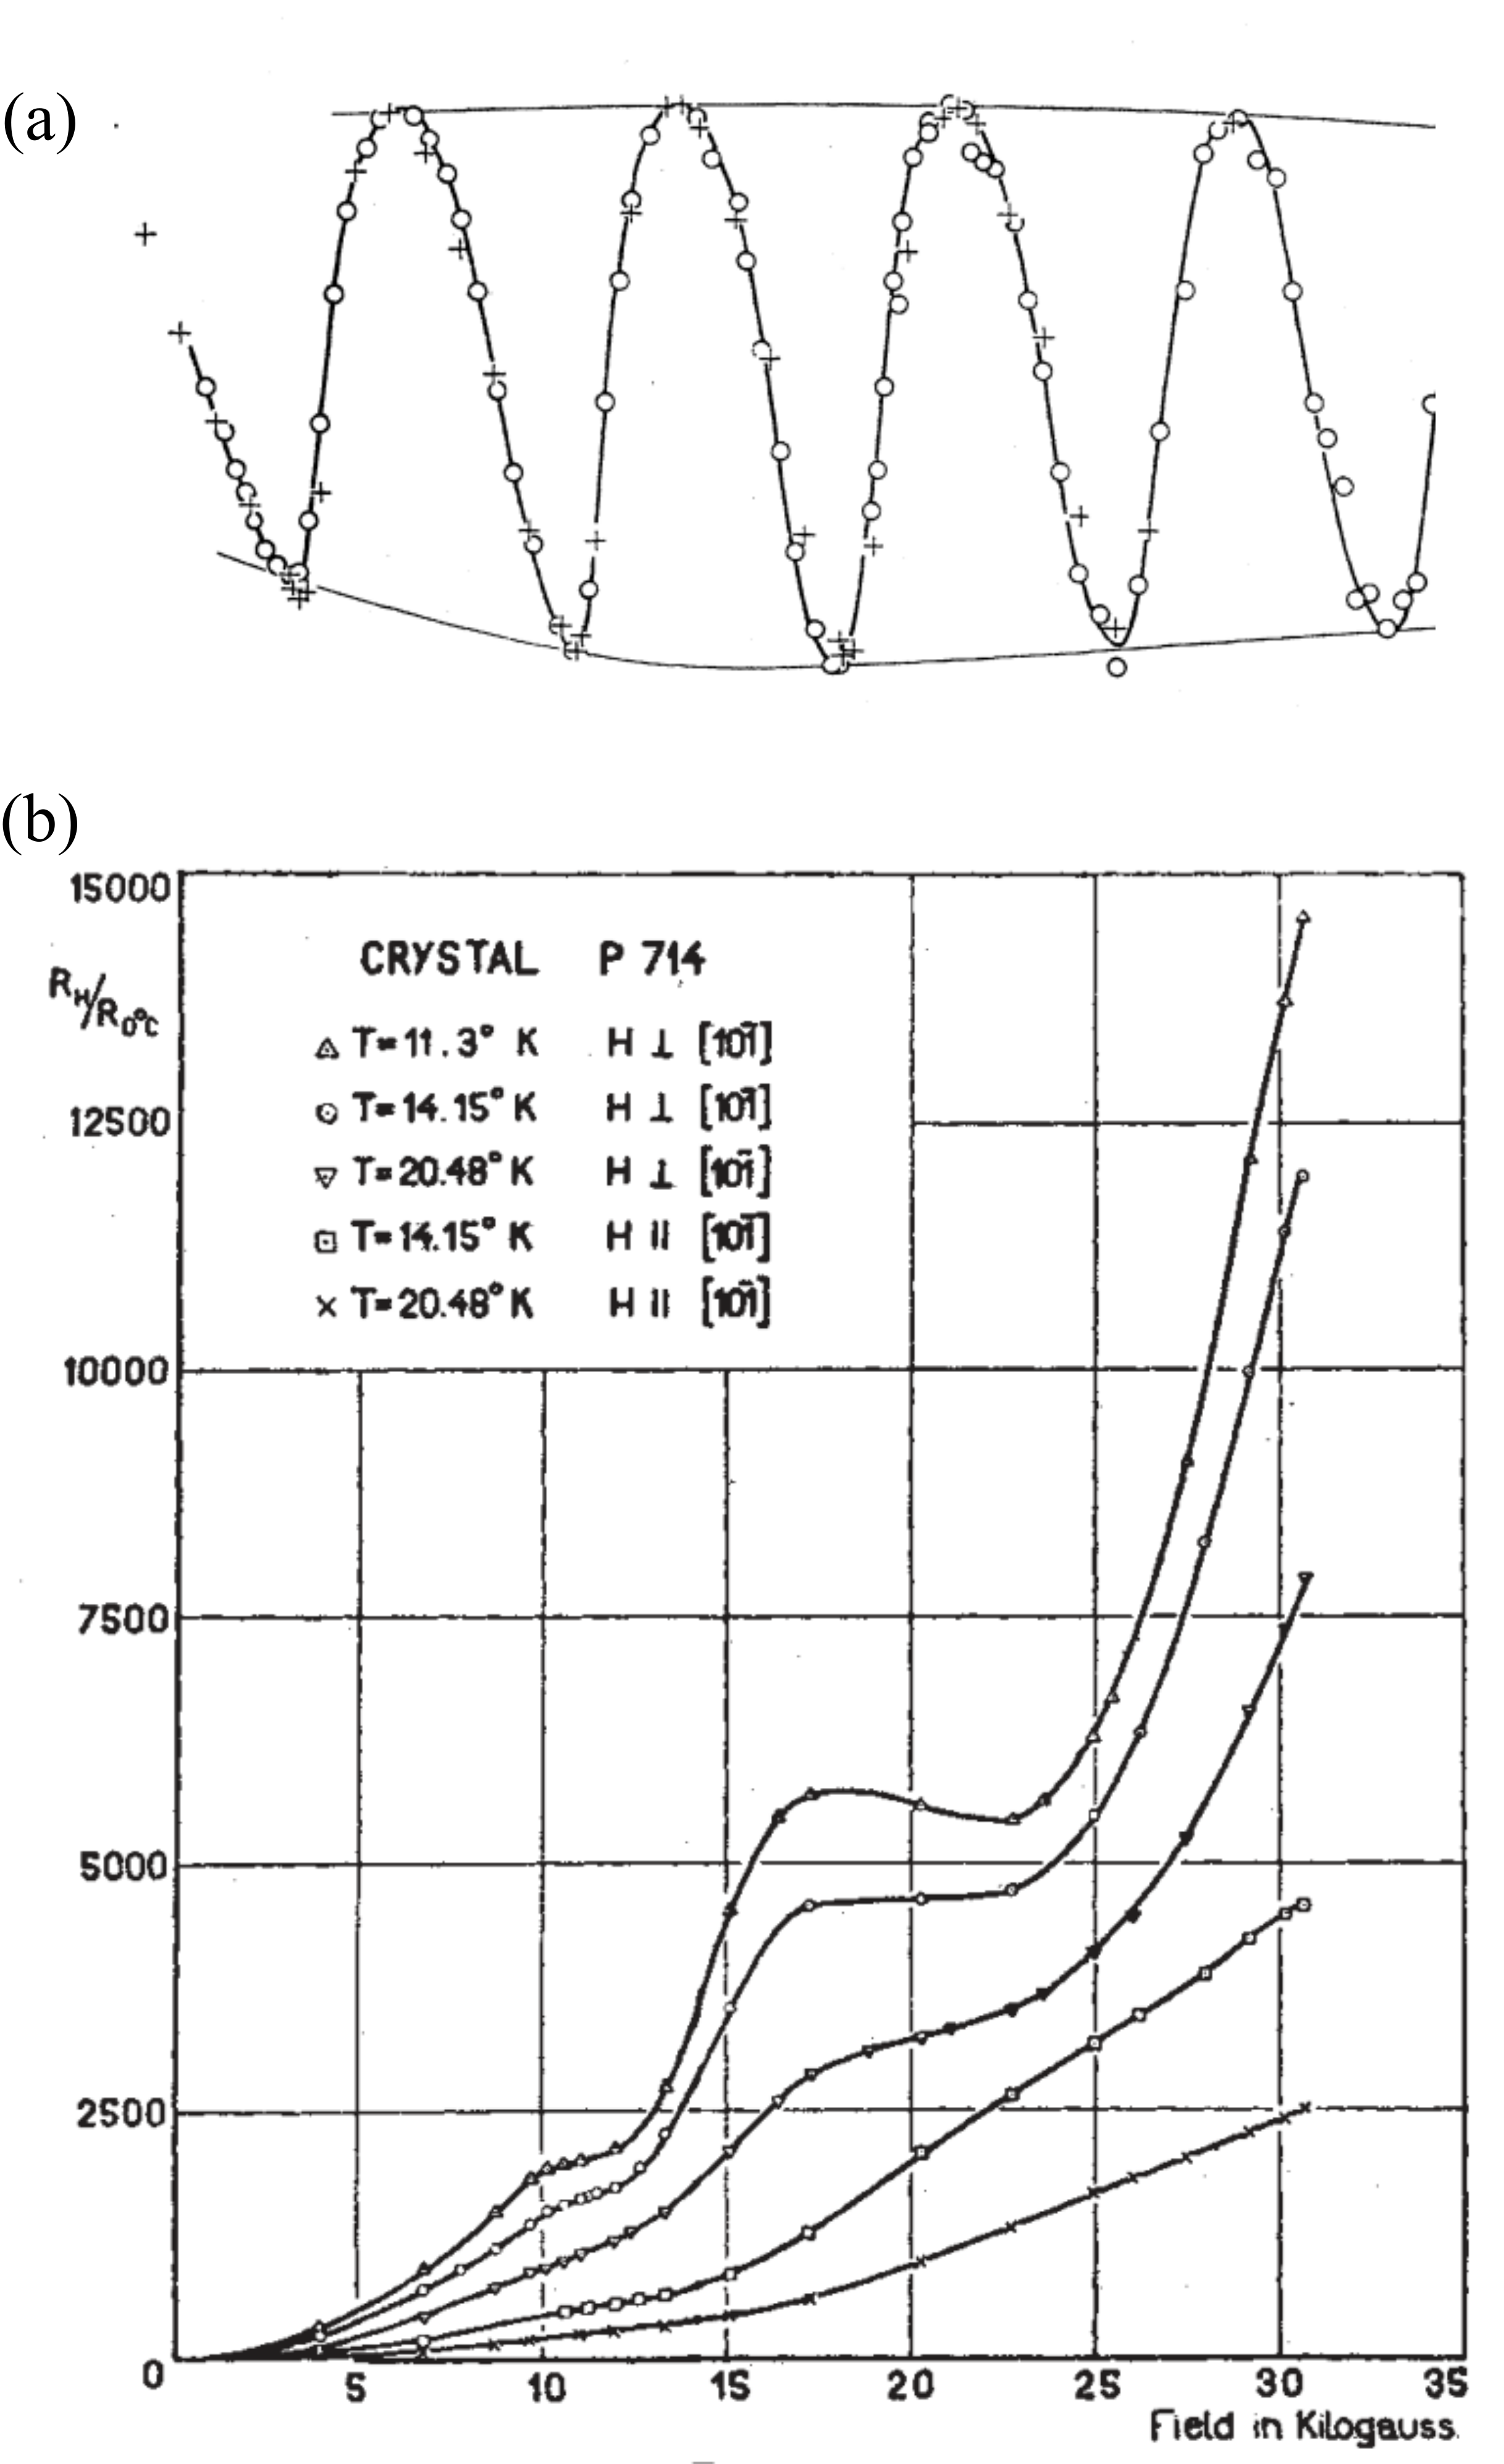
\includegraphics[width=1.0\textwidth]{../figures/quantum-oscillation.png}
	\caption{dHvA振荡(a)和SdH振荡(b). (a)图中横坐标为磁场,纵坐标为$\delta M/B$.\label{quantum-oscillation}}
\end{figure}

量子振荡的基本起源是朗道能级的分立性。随着磁场的变化,朗道能级的能量也会发生变化。当朗道能级穿过费米面的时候,材料的各种性质都会发生比较明显的变化,从而产生振荡效应。将式\ref{single-quan}中的能量取定为费米能,我们可以得到,朗道能级穿过费米面这一事件是随着$l^2$,也就是$1/B$周期发生的,因此量子振荡是随着$1/B$周期性振荡的。

Landau和Lifshitz给出了量子振荡的具体的表达式。一般而言,我们认为电阻正比于费米面处的态密度,所以SdH振荡就正比于态密度振荡。在费米面附近态密度振荡部分的表达式为
\begin{equation}
\delta\nu (E) = \left. \frac{1}{4\pi^3}\frac{\hbar^2}{m_c}\left(\frac{\partial S}{\partial E}\right)^2\sum_{r=1}^{\infty} e^{-r\pi/\omega_c\tau}
\cos [r(l^2 S+\lambda+\pi)] \right|_{E=E_F}.
\end{equation}
这里, $\tau$是Diggle散射时长,代表了杂质的作用。所有的量都是在费米能处计算的。

对于dHvA振荡而言,磁矩的振荡来源于自由能的振荡
\begin{equation}
\delta M = \left. -\frac{1}{2\pi}\frac{k_B T}{B} S\sum_{r=1}^{\infty}e^{-r\pi/\omega_c\tau}\frac{\sin[r(l^2 S+\lambda+\pi)]}{\sinh(2\pi^2 r k_B T/\hbar \omega_c)}\right|_{E=E_F}.
\end{equation}
这里$T$是温度,$k_B$是玻尔兹曼常数。

一般而言,在实验条件下,只有最低阶的振荡($r=1$的振荡)可以被观察到。这种情况下,dHvA振荡和SdH振荡的周期都是反比于费米圆的面积。因此,量子振荡最重要的应用便是测量费米圆的大小。除此之外,我们看到$\lambda$在量子振荡中表现为相位,因此,$\lambda$也是一个可以测量的物理量。$\lambda$体现了费米面处波函数的拓扑性质,近些年来为实验所关注。